\begin{figure}[H]
   \centering
   % Fila 1: el grafo y el archivo, centrados verticalmente
   \begin{minipage}[c]{0.40\textwidth}
      \centering
      \resizebox{0.78\linewidth}{!}{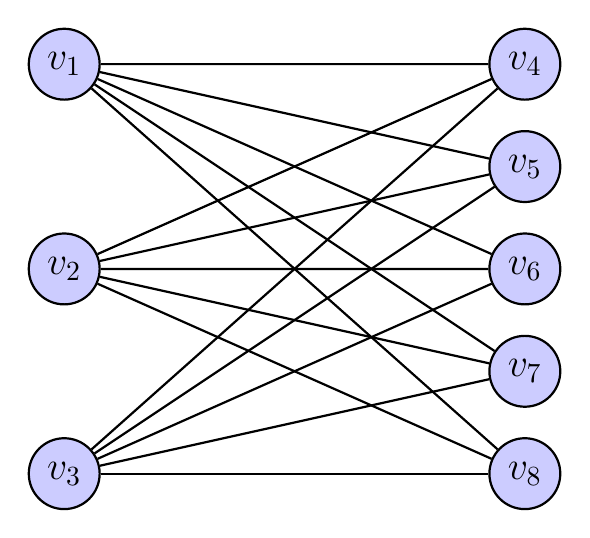
\begin{tikzpicture}[
  scale=1.3,
  vnode/.style={circle, fill=blue!20, draw=black, thick, minimum size=9mm, inner sep=0pt, font=\Large}
]
  % Partición izquierda
  \node[vnode] (v1) at (0, 4) {$v_1$};
  \node[vnode] (v2) at (0, 2) {$v_2$};
  \node[vnode] (v3) at (0, 0) {$v_3$};

  % Partición derecha
  \foreach \j in {4,...,8} {
    \node[vnode] (v\j) at (4.5, {8-\j}) {$v_{\j}$};
  }

  % Aristas: cada vértice de la izquierda con cada vértice de la derecha
  \foreach \i in {1,2,3} {
    \foreach \j in {4,...,8} {
      \draw[thick] (v\i) -- (v\j);
    }
  }
\end{tikzpicture}
}
   \end{minipage}%
   \hspace{1.5em}%
   \begin{minipage}[c]{0.42\textwidth}
\begin{lstlisting}[framexrightmargin=-4.4pt]
8 (*@\label{lin:r1_2_Mat_Ady}@*)
0 0 0 1 1 1 1 1 (*@\label{lin:inicio_2_Mat_Ady}@*)
0 0 0 1 1 1 1 1
0 0 0 1 1 1 1 1
1 1 1 0 0 0 0 0
1 1 1 0 0 0 0 0
1 1 1 0 0 0 0 0
1 1 1 0 0 0 0 0
1 1 1 0 0 0 0 0 (*@\label{lin:fin_2_Mat_Ady}@*)
\end{lstlisting}
\end{minipage}

   % Fila 2: los pies, alineados arriba y centrados
   \captionsetup{format=plain, justification=centering}
   \begin{minipage}[t]{0.40\textwidth}
      \captionof{figure}{Grafo $K_{3,5}$}
      \label{fig:K_3,5}
   \end{minipage}%
   \hspace{1.5em}%
   \begin{minipage}[t]{0.42\textwidth}
      \captionof{lstlisting}{Archivo \texttt{2\_Mat\_Ady.txt} para guardar la información de $K_{3,5}$}
      \label{cod:2_Mat_Ady}
   \end{minipage}
\end{figure}
